\documentclass[conference]{IEEEtran}

% --- Encoding / fuentes ---
\usepackage[utf8]{inputenc}
\usepackage[T1]{fontenc}

% --- Utilidades básicas ---
\usepackage{graphicx}
\usepackage{amsmath, amssymb}
\usepackage{cite}
\usepackage{url}
\usepackage{microtype} % opcional, recomendado
\usepackage{subfig}
% Requiere en el preámbulo:
% \usepackage{subfig}
\usepackage{tikz}
\usetikzlibrary{positioning,arrows.meta,calc}

% --- TikZ (pipeline) + TikZ-CD (diagramas conmutativos) ---
\usepackage{tikz}
\usetikzlibrary{arrows.meta,positioning,shapes.geometric,calc}
\usepackage{tikz-cd}
\usepackage{adjustbox}
\usepackage{float}    
\usepackage{placeins}  


\title{Segmentación automática de columna vertebral y vértebras en radiografías con escoliosis para entornos con recursos computacionales limitados}

\author{
\IEEEauthorblockN{Jason Rosher Morrill, John Williams Morrill, David Alan Delgado Zarco, Octavio Esquivel Álvarez del Castillo}
\IEEEauthorblockA{Maestría en Inteligencia Artificial (MAIA)\\
Universidad de los Andes, Bogotá, Colombia\\
j.morrill@uniandes.edu.co, j.williams@uniandes.edu.co, d.delgado@uniandes.edu.co, o.esquivel@uniandes.edu.co}
}

\begin{document}
\maketitle

\begin{abstract}

La segmentación automática de la columna vertebral en radiografías es una tarea compleja debido a la superposición de estructuras anatómicas, variabilidad morfológica y limitaciones en la calidad de las imágenes. Los métodos actuales basados en redes convolucionales y Transformers han mostrado buenos resultados en tomografía computarizada, pero su aplicación en radiografías 2D sigue siendo limitada y depende frecuentemente de postprocesamientos heurísticos.

En este trabajo se propone un modelo híbrido que combina redes convolucionales, análisis topológico de datos (TDA) y Transformers con atención kernelizada para mejorar la segmentación vertebral. El modelo incorpora descriptores topológicos y geométricos en el espacio de representación, permitiendo capturar simultáneamente información local, global y estructural.

La arquitectura propuesta introduce un Transformer multi-kernel donde cada cabeza de atención opera sobre distintos espacios de representación (CNN, topológico y manifold). Este enfoque busca mejorar la coherencia anatómica de la segmentación en radiografías con escoliosis.

El trabajo presenta el marco teórico y la metodología propuesta para integrar geometría diferencial y análisis topológico dentro de arquitecturas profundas para segmentación médica.

\end{abstract}

\begin{IEEEkeywords}
spine, vertebra segmentation, transformer, topological data analysis, persistent homology, differential geometry
\end{IEEEkeywords}

\section{Introducción}

\section{Estado del Arte}
\label{sec:sota}

La segmentación automática de columna y vértebras ha evolucionado rápidamente con arquitecturas profundas que combinan extracción local de rasgos y modelado de contexto global. En tomografía computarizada (CT) 3D, predominan enfoques tipo U-Net y variantes modernas (p.ej., nnU-Net), que han establecido baselines fuertes para segmentación vertebral multi-etiqueta. Más recientemente, los Transformers se han incorporado para capturar dependencias de largo alcance y mejorar la consistencia anatómica, especialmente en escenarios de \emph{arbitrary field-of-view} (FOV) donde el número de vértebras visibles y su escala varían.

En el contexto Transformer, se observan dos tendencias principales. La primera adopta paradigmas tipo DETR para tratar la detección/etiquetado vertebral como un problema de predicción de conjuntos mediante \emph{query tokens} (consultas aprendibles) asociados a instancias anatómicas, que luego guían etapas de segmentación. La segunda integra Transformers (ViT/Swin) dentro de arquitecturas encoder--decoder tipo U-Net, operando sobre \emph{patch tokens} o \emph{feature tokens} para proveer contexto global en la segmentación densa. En varios trabajos, la \emph{anatomy-awareness} se introduce mediante tareas auxiliares y regularizadores geométricos simples, por ejemplo: módulos de detección de bordes para reforzar la separación entre vértebras adyacentes, o aprendizaje multi-tarea con detección de centroides que aporta una señal global de localización y reduce errores en vértebras terminales o raras.

Sin embargo, pese a estos avances, la información geométrica y topológica incorporada en la mayoría de métodos es limitada. En general, la ``geometría'' se reduce a cajas, centroides, mapas de borde o codificaciones posicionales estándar, sin incluir descriptores formales de geometría diferencial (curvatura, geodésicas) ni resúmenes topológicos provenientes de TDA (p. ej., homología persistente, números de Betti, \emph{persistence diagrams/images}). Esto es particularmente notorio en radiografías 2D (X-ray), donde los trabajos basados en Transformers son escasos y suelen depender de postprocesamientos heurísticos para corregir fusiones o incongruencias entre vértebras. En consecuencia, existe una oportunidad clara para modelos que representen explícitamente cada vértebra como un token anatómico enriquecido con descriptores topológicos y geométricos, y que utilicen atención informada por estructura (adyacencia anatómica, distancias geodésicas, perfil de curvatura) para mejorar la fidelidad anatómica de la segmentación en X-ray.

\begin{table*}[t]
\centering
\caption{Resumen comparativo de enfoques recientes basados en Transformers para segmentación de columna/vértebras y el vacío que aborda la propuesta.}
\label{tab:sota_summary}
\resizebox{\textwidth}{!}{%
\begin{tabular}{p{2.2cm} p{2.1cm} p{2.2cm} p{2.9cm} p{2.9cm} p{3.6cm}}
\hline
\textbf{Familia / Idea} &
\textbf{Modalidad típica} &
\textbf{Tokens en Transformer} &
\textbf{Señal anatómica/geométrica usada} &
\textbf{Limitación principal} &
\textbf{Cómo se conecta con nuestra propuesta} \\
\hline

DETR/queries para vértebras (detección--etiquetado $\rightarrow$ segmentación) &
CT 3D (arbitrary FOV) &
\emph{Query tokens} (instancia-like) &
Relaciones globales vía atención + codificación posicional; geometría implícita (centros/cajas/esferas/pose) &
Las queries no incorporan TDA/curvatura/geodésicas; la topología no entra al embedding ni a la atención &
Reutilizamos la idea de \emph{tokens anatómicos} pero los definimos por vértebra y los enriquecemos con TDA/geo \\
\hline

ViT/Swin + U-Net (segmentación densa single-stage) &
CT 3D (multi-label), algunas variantes 2D &
\emph{Patch/feature tokens} &
Contexto global; a veces manejo de FOV; priors anatómicos implícitos por supervisión &
No hay tokens por vértebra; ``estructura'' aprendida es implícita; sin atención informada por cadena vertebral &
Proponemos pasar de patches a \emph{tokens por vértebra} y usar atención estructurada por anatomía \\
\hline

Refinamiento por bordes (edge modules + loss) &
CT 3D &
Patch/feature tokens (Transformer) + módulos CNN &
Mapas de bordes / contornos para separar vértebras y afinar límites &
Regularización local; no modela topología global ni relaciones vertebra--vertebra (geodésicas/curvatura) &
Complementamos bordes con descriptores TDA/geo y atención sesgada por adyacencia \\
\hline

Multi-tarea con centroides (centroid-guided) &
CT 2D (sagital/coronal), CT 3D; transferible a X-ray &
Patch/feature tokens; centroides como señal auxiliar &
Centroides/heatmaps guían segmentación; algunas pérdidas con restricciones anatómicas &
No formaliza geodésicas/curvatura; no hay embeddings topológicos por vértebra &
Usamos centroides/ROIs para construir tokens por vértebra y añadir descriptores TDA/geo \\
\hline

Transformers en X-ray 2D (segmentación genérica + postproceso) &
X-ray 2D &
Patch tokens &
Postprocesamiento heurístico para separar regiones fusionadas &
Muy poca anatomía explícita; topología corregida fuera del modelo &
Objetivo: eliminar heurísticas integrando tokens vertebrales + TDA/geo dentro del modelo \\
\hline

\textbf{Vacío (gap)} &
\textbf{X-ray 2D (nuestro foco)} &
\textbf{Tokens por vértebra} &
\textbf{TDA (persistencia/Betti) + geometría (curvatura/geodésicas) + sesgos de atención por adyacencia} &
\textbf{No reportado como combinación integrada en la literatura reciente} &
\textbf{Propuesta: vertebra-tokens enriquecidos $\rightarrow$ Transformer multi-kernel $\rightarrow$ decoder denso} \\
\hline
\end{tabular}%
}
\end{table*}

\section{Marco Teórico}

\subsection{Redes Convolucionales para Segmentación Médica}

\subsection{Transformers en Visión Computacional}

\subsection{Análisis Topológico de Datos}

\subsection{Geometría Diferencial en Representaciones de Datos}

\section{Metodología Propuesta}

\subsection{Visión General}

Se propone un pipeline híbrido que combina redes convolucionales (CNN), análisis topológico de datos (TDA) y modelos tipo Transformer. La idea central consiste en enriquecer la representación de las imágenes médicas incorporando información tanto local como global, topológica y geométrica, con el objetivo de mejorar la segmentación de la columna vertebral y sus vértebras.

Formalmente, la imagen de entrada se modela como una función:
\[
x : \Omega \rightarrow \mathbb{R}
\]
donde $\Omega \subset \mathbb{R}^2$ es el dominio espacial de la radiografía.

El flujo general del modelo es el siguiente:

\begin{center}
\texttt{Imagen $\rightarrow$ CNN $\rightarrow$ Feature Maps $\rightarrow$ Enriquecimiento Topológico $\rightarrow$ Transformer Multi-kernel $\rightarrow$ Segmentación}
\end{center}

\subsection{Diagrama del Pipeline}

\begin{center}
\resizebox{\columnwidth}{!}{%
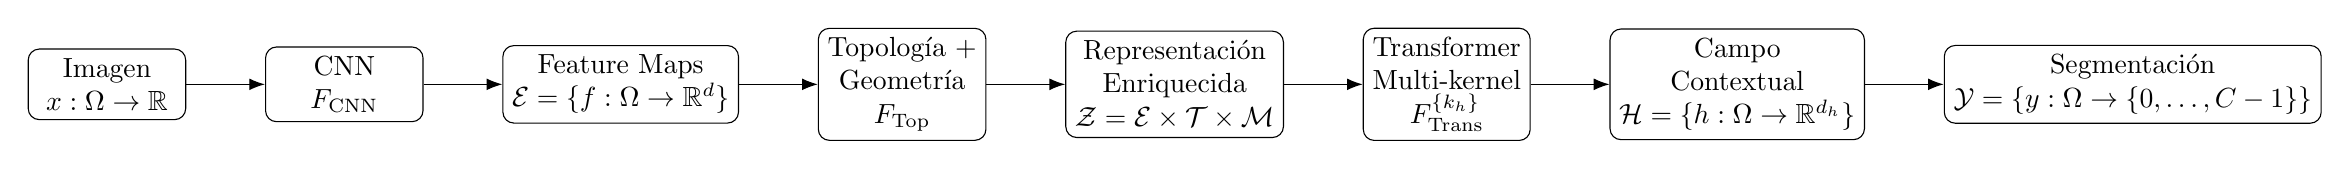
\begin{tikzpicture}[
  node distance=10mm,
  every node/.style={
    draw, rectangle, rounded corners,
    minimum width=20mm, minimum height=7mm,
    align=center
  }
]

\node (input) {Imagen\\$x:\Omega\to\mathbb{R}$};

\node (cnn) [right=of input] {CNN\\$F_{\text{CNN}}$};

\node (E) [right=of cnn] {Feature Maps\\$\mathcal{E}=\{f:\Omega\to\mathbb{R}^d\}$};

\node (top) [right=of E] {Topología +\\Geometría\\$F_{\text{Top}}$};

\node (Z) [right=of top] {Representación\\Enriquecida\\$\mathcal{Z}=\mathcal{E}\times\mathcal{T}\times\mathcal{M}$};

\node (trans) [right=of Z] {Transformer\\Multi-kernel\\$F_{\text{Trans}}^{\{k_h\}}$};

\node (H) [right=of trans] {Campo\\Contextual\\$\mathcal{H}=\{h:\Omega\to\mathbb{R}^{d_h}\}$};

\node (out) [right=of H] {Segmentación\\$\mathcal{Y}=\{y:\Omega\to\{0,\dots,C-1\}\}$};

\draw[-{Latex[length=2mm]}] (input) -- (cnn);
\draw[-{Latex[length=2mm]}] (cnn) -- (E);
\draw[-{Latex[length=2mm]}] (E) -- (top);
\draw[-{Latex[length=2mm]}] (top) -- (Z);
\draw[-{Latex[length=2mm]}] (Z) -- (trans);
\draw[-{Latex[length=2mm]}] (trans) -- (H);
\draw[-{Latex[length=2mm]}] (H) -- (out);

\end{tikzpicture}%
}
\end{center}

\subsection{Interpretación}

Cada bloque del pipeline puede interpretarse como una transformación entre espacios estructurados:

\begin{itemize}
    \item $\mathcal{X}$: espacio de imágenes (funciones sobre $\Omega$)
    \item $\mathcal{E}$: tensores (feature maps)
    \item $\mathcal{T}$: descriptores topológicos (homología persistente)
    \item $\mathcal{M}$: estructura geométrica (manifold)
    \item $\mathcal{Z}$: representación enriquecida
    \item $\mathcal{H}$: campos vectoriales contextualizados
    \item $\mathcal{Y}$: segmentación por píxel (vértebra a vértebra)
\end{itemize}

El modelo completo se expresa como:
\[
F = F_{\text{Dec}} \circ F_{\text{Trans}}^{\{k_h\}} \circ F_{\text{Top}} \circ F_{\text{CNN}}
\]

\subsection{Asignación de Kernels por Espacio}

El Transformer propuesto no utiliza únicamente el producto punto, sino que cada cabeza de atención opera con un kernel específico dependiendo del espacio de representación.

\begin{center}
\resizebox{\columnwidth}{!}{%
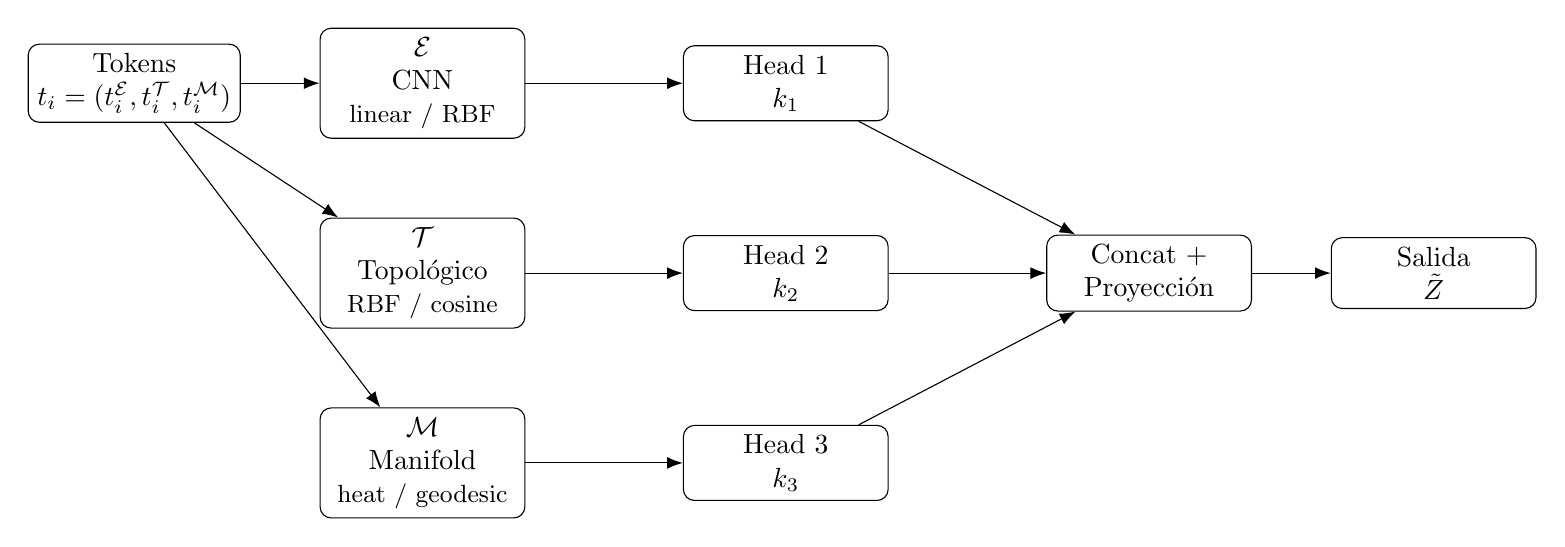
\begin{tikzpicture}[
  node distance=10mm,
  every node/.style={
    draw, rounded corners,
    minimum width=26mm, minimum height=8mm,
    align=center
  }
]

\node (tokens) {Tokens\\$t_i=(t_i^{\mathcal{E}},t_i^{\mathcal{T}},t_i^{\mathcal{M}})$};

\node (E) [right=of tokens] {$\mathcal{E}$\\CNN\\\small linear / RBF};
\node (T) [below=of E] {$\mathcal{T}$\\Topológico\\\small RBF / cosine};
\node (M) [below=of T] {$\mathcal{M}$\\Manifold\\\small heat / geodesic};

\node (h1) [right=20mm of E] {Head 1\\$k_1$};
\node (h2) [right=20mm of T] {Head 2\\$k_2$};
\node (h3) [right=20mm of M] {Head 3\\$k_3$};

\node (mix) [right=20mm of h2] {Concat +\\Proyección};
\node (out) [right=of mix] {Salida\\$\tilde{Z}$};

\draw[-{Latex[length=2mm]}] (tokens) -- (E);
\draw[-{Latex[length=2mm]}] (tokens) -- (T);
\draw[-{Latex[length=2mm]}] (tokens) -- (M);

\draw[-{Latex[length=2mm]}] (E) -- (h1);
\draw[-{Latex[length=2mm]}] (T) -- (h2);
\draw[-{Latex[length=2mm]}] (M) -- (h3);

\draw[-{Latex[length=2mm]}] (h1) -- (mix);
\draw[-{Latex[length=2mm]}] (h2) -- (mix);
\draw[-{Latex[length=2mm]}] (h3) -- (mix);

\draw[-{Latex[length=2mm]}] (mix) -- (out);

\end{tikzpicture}%
}
\end{center}

\subsection{Interpretación del Transformer}

El Transformer actúa como un operador que genera un campo contextual sobre la imagen:
\[
F_{\text{Trans}}^{\{k_h\}} : \mathcal{Z} \rightarrow \mathcal{H}
\]

donde cada cabeza implementa una noción distinta de similitud estructural mediante kernels. Esto permite capturar simultáneamente relaciones:

\begin{itemize}
    \item locales (CNN),
    \item globales (atención),
    \item topológicas (TDA),
    \item geométricas (manifold).
\end{itemize}



\subsection{Extracción de Características con CNN}

Sea $x \in \mathcal{X}$ una imagen de entrada. Se utiliza una red convolucional para extraer características locales:
\[
F_{\text{CNN}}: \mathcal{X} \rightarrow \mathcal{E}
\]
donde $\mathcal{E} \subset \mathbb{R}^d$ es el espacio de embeddings.

\subsection{Enriquecimiento Topológico}

El embedding $z \in \mathcal{E}$ se transforma para incorporar información estructural global mediante herramientas topológicas.

\subsubsection{Construcción de Complejo Simplicial}
\[
F_{\text{simp}}: \mathcal{E} \rightarrow \mathcal{S}
\]

\subsubsection{Extracción de Características Topológicas (TDA)}
\[
F_{\text{TDA}}: \mathcal{S} \rightarrow \mathcal{T}
\]

\subsubsection{Suposición de Manifold}
\[
F_{\text{man}}: \mathcal{E} \rightarrow \mathcal{M}
\]

\subsection{Representación Enriquecida}
\[
z_{\text{enriquecido}} = \text{concat}(z_{\text{CNN}}, z_{\text{TDA}}, z_{\text{manifold}})
\]

\subsection{Transformer Multi-kernel en Espacios Múltiples}

A diferencia de un Transformer estándar (atención por producto punto), proponemos un bloque de atención donde cada cabeza opera con una noción de similitud dada por un \emph{kernel}. La motivación es que distintos kernels pueden capturar mejor relaciones en diferentes espacios: euclídeo (CNN), topológico (TDA) y geométrico (manifold).

Sea $Z = \{t_i\}_{i=1}^{n}$ la secuencia de tokens derivada de $z_{\text{enriquecido}}$. Para cada cabeza $h \in \{1,\dots,H\}$ se define un kernel $k_h(\cdot,\cdot)$, y se construye una matriz de afinidad $K_h \in \mathbb{R}^{n\times n}$:
\[
(K_h)_{ij} = k_h(t_i,t_j).
\]
Los pesos de atención se obtienen normalizando por fila:
\[
A_h(i,j) = \frac{\exp((K_h)_{ij})}{\sum_{j'=1}^{n}\exp((K_h)_{ij'})}.
\]
La salida por cabeza se calcula como:
\[
\mathrm{head}_h(i) = \sum_{j=1}^{n} A_h(i,j)\,V_h(t_j),
\]
y el bloque multi-cabeza se obtiene por concatenación y proyección:
\[
\mathrm{MHA}(t_i)=W_O\,[\mathrm{head}_1(i)\,\|\,\cdots\,\|\,\mathrm{head}_H(i)].
\]

\subsubsection{Asignación de kernels por espacio}

Se define un conjunto finito de kernels candidatos $\mathcal{K}$ (p.ej., lineal, RBF, polinomial, coseno). Cada kernel se asocia a un espacio de representación:

\begin{itemize}
    \item $\mathcal{E}$ (CNN): kernels sobre $z_{\text{CNN}} \in \mathbb{R}^{d}$.
    \item $\mathcal{T}$ (TDA): kernels sobre descriptores topológicos vectorizados $z_{\text{TDA}}$.
    \item $\mathcal{M}$ (manifold): kernels sobre coordenadas/embeddings que preservan geometría local.
\end{itemize}

\subsubsection{Exploración y ablación}

Se propone evaluar configuraciones donde:
\begin{itemize}
    \item todas las cabezas usan el mismo kernel ($k_h \equiv k$),
    \item las cabezas se reparten entre kernels ($k_h \in \mathcal{K}$),
    \item comparación contra atención estándar (producto punto).
\end{itemize}

\subsubsection{Aproximación Nyström (opcional)}

Para reducir el costo cuando $n$ es grande, se plantea aproximar $K_h$ con Nyström:
\[
K_h \approx C_h\,W_h^{\dagger}\,C_h^\top,
\]
donde $r \ll n$ es el número de anclas. Esto preserva la estructura kernelizada con menor complejidad.

\subsubsection{Diagrama del Bloque de Atención Multi-kernel}

\begin{center}
\resizebox{\columnwidth}{!}{%
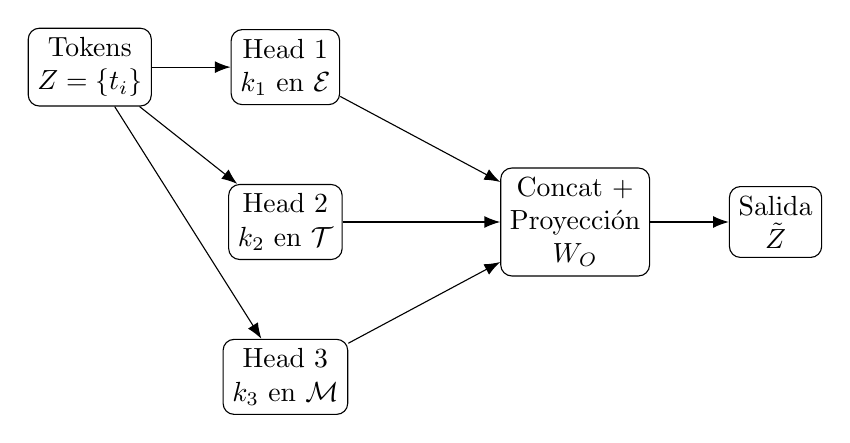
\begin{tikzpicture}[
  every node/.style={draw, rounded corners, align=center, minimum height=7mm},
  node distance=10mm
]
\node (tokens) {Tokens\\$Z=\{t_i\}$};

\node (h1) [right=of tokens] {Head 1\\$k_1$ en $\mathcal{E}$};
\node (h2) [below=of h1] {Head 2\\$k_2$ en $\mathcal{T}$};
\node (h3) [below=of h2] {Head 3\\$k_3$ en $\mathcal{M}$};

\node (mix) [right=20mm of h2] {Concat +\\Proyección\\$W_O$};
\node (out) [right=of mix] {Salida\\$\tilde{Z}$};

\draw[-{Latex[length=2mm]}] (tokens) -- (h1);
\draw[-{Latex[length=2mm]}] (tokens) -- (h2);
\draw[-{Latex[length=2mm]}] (tokens) -- (h3);

\draw[-{Latex[length=2mm]}] (h1) -- (mix);
\draw[-{Latex[length=2mm]}] (h2) -- (mix);
\draw[-{Latex[length=2mm]}] (h3) -- (mix);

\draw[-{Latex[length=2mm]}] (mix) -- (out);
\end{tikzpicture}%
}
\end{center}

\subsection{Procesamiento con Transformer}
\[
F_{\text{Trans}}: \mathcal{Z} \rightarrow \mathcal{Y}
\]

\subsection{Interpretación Categórica}

El pipeline completo puede interpretarse como la composición de transformaciones entre espacios estructurados:
\[
F = F_{\text{Trans}} \circ F_{\text{Top}} \circ F_{\text{CNN}}
\]


\subsection{Diagrama Funtorial}

\begin{center}
\begin{adjustbox}{max width=\columnwidth}
\begin{tikzcd}
\mathcal{X} \arrow[r, "F_{\text{CNN}}"] &
\mathcal{E} \arrow[r, "F_{\text{Top}}"] &
\mathcal{Z} \arrow[r, "F_{\text{Trans}}"] &
\mathcal{Y}
\end{tikzcd}
\end{adjustbox}
\end{center}

donde:
\begin{itemize}
\item $\mathcal{X}$: espacio de imágenes
\item $\mathcal{E}$: espacio de embeddings
\item $\mathcal{Z}$: representación enriquecida
\item $\mathcal{Y}$: espacio de salida
\end{itemize}

\subsection{Descomposición del Funtor Topológico}

El enriquecimiento topológico se descompone como:
\[
F_{\text{Top}} = F_{\text{TDA}} \circ F_{\text{simp}} \circ F_{\text{man}}
\]

\begin{center}
\begin{adjustbox}{max width=\columnwidth}
\begin{tikzcd}
\mathcal{E} \arrow[r, "F_{\text{simp}}"] &
\mathcal{S} \arrow[r, "F_{\text{TDA}}"] &
\mathcal{T}
\end{tikzcd}
\end{adjustbox}
\end{center}

\subsection{Tarea de Salida}
Dependiendo del problema, la salida $\mathcal{Y}$ puede representar:
\begin{itemize}
\item Segmentación de la columna
\item Clasificación de severidad
\item Estimación del ángulo de Cobb
\end{itemize}

\subsection{Dataset}

El dataset utilizado contiene radiografías anteroposteriores de columna vertebral
correspondientes a pacientes con y sin escoliosis. Cada imagen incluye diferentes
niveles de anotación que permiten analizar la estructura anatómica de la columna.

Las representaciones disponibles incluyen:

\begin{itemize}

\item \textbf{Radiografía original}: imagen médica en escala de grises.

\item \textbf{Máscara binaria}: segmentación de la columna vertebral donde los
píxeles pertenecientes a la columna toman valor 255 y el resto corresponde al fondo.

\item \textbf{Segmentación multiclase}: cada vértebra se representa con una etiqueta
independiente (por ejemplo C7, T1--T12, L1--L5).

\item \textbf{Curva espinal}: línea central de la columna estimada a partir de la
máscara segmentada.

\item \textbf{Métricas clínicas}: cálculo automático del ángulo de Cobb,
utilizado para cuantificar la severidad de la escoliosis.

\end{itemize}

\begin{figure}[!t]
\centering
\setlength{\tabcolsep}{3pt}

\begin{tabular}{cc}
\subfloat[Radiografía AP]{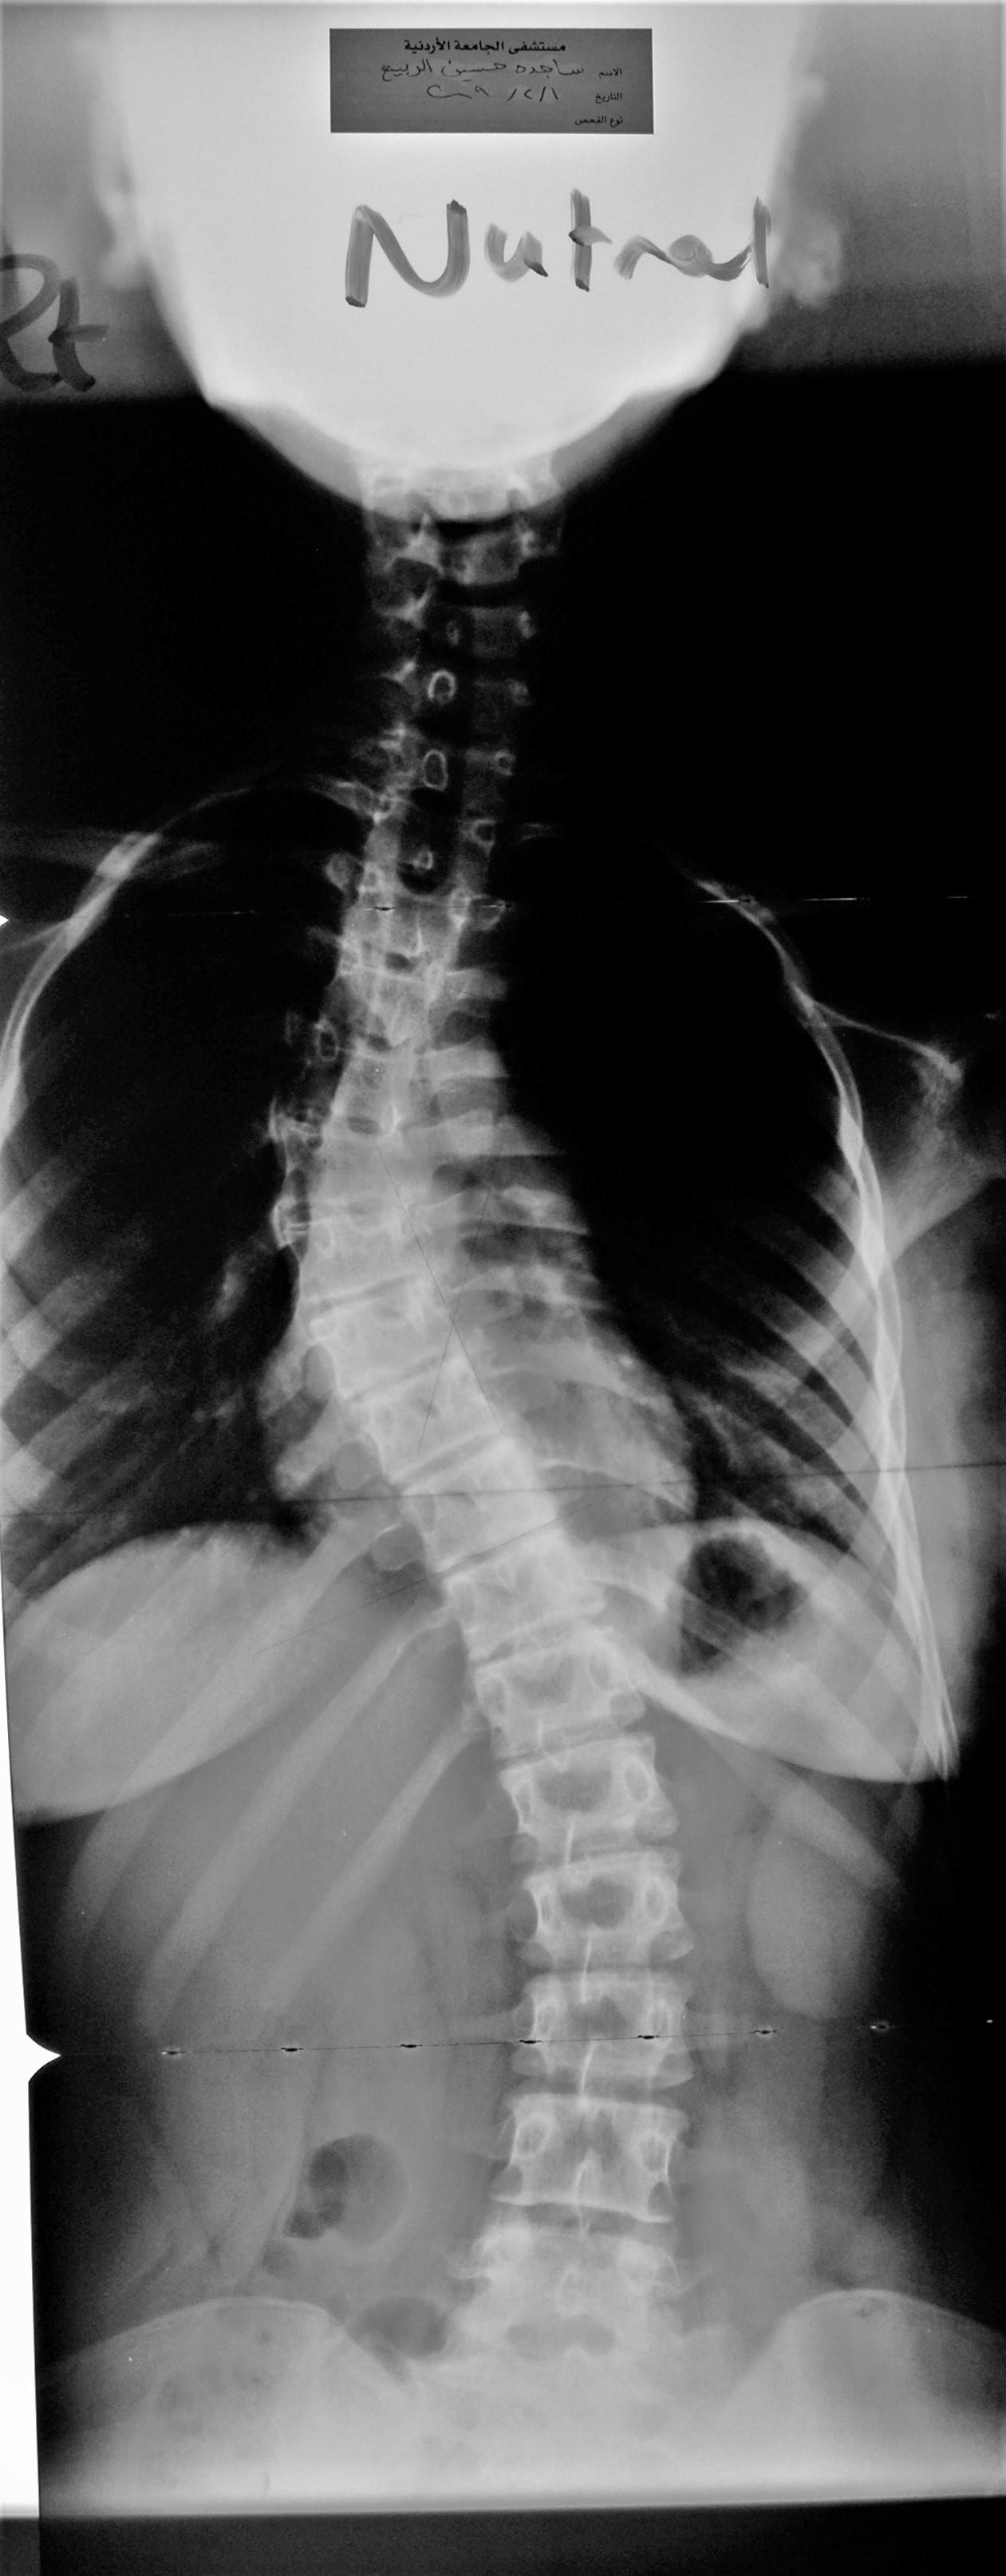
\includegraphics[width=0.27\linewidth]{imagenes/S_94.jpg}} &
\subfloat[Segmentación multiclase]{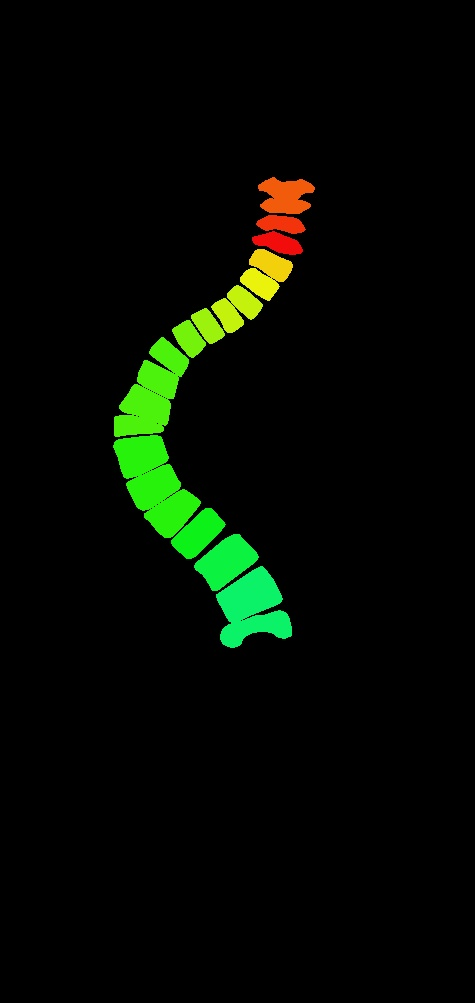
\includegraphics[width=0.27\linewidth]{imagenes/LabelMulti_S_64.jpg}}
\end{tabular}

\caption{Ejemplos del dataset: (a) radiografía anteroposterior de columna
y (b) segmentación multiclase de las vértebras.}

\label{fig:dataset_images}

\end{figure}

A partir de la segmentación es posible obtener representaciones geométricas
de la columna vertebral. En particular, se puede estimar la línea central
de la columna y calcular métricas clínicas como el ángulo de Cobb, ampliamente
utilizado en la práctica médica para evaluar la severidad de la escoliosis.

\begin{figure}[!t]
\centering
\setlength{\tabcolsep}{3pt}

\begin{tabular}{cc}
\subfloat[Línea central estimada]{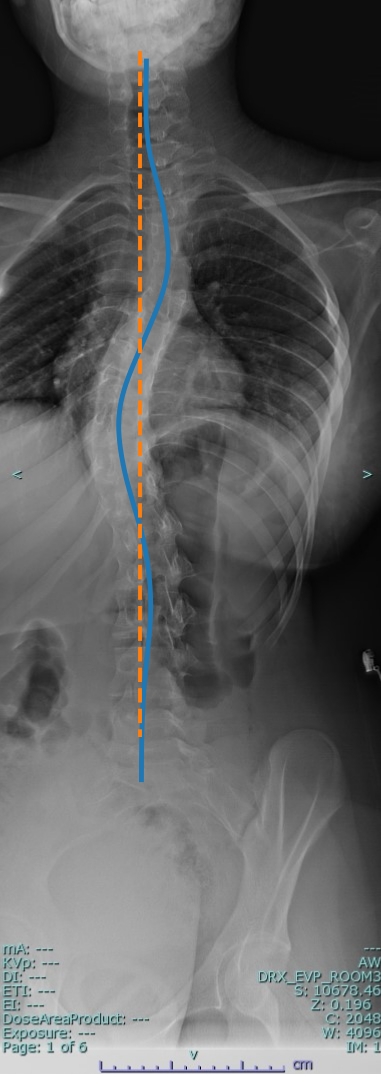
\includegraphics[width=0.27\linewidth]{imagenes/overlay_21.png}} &
\subfloat[Métricas clínicas (Cobb)]{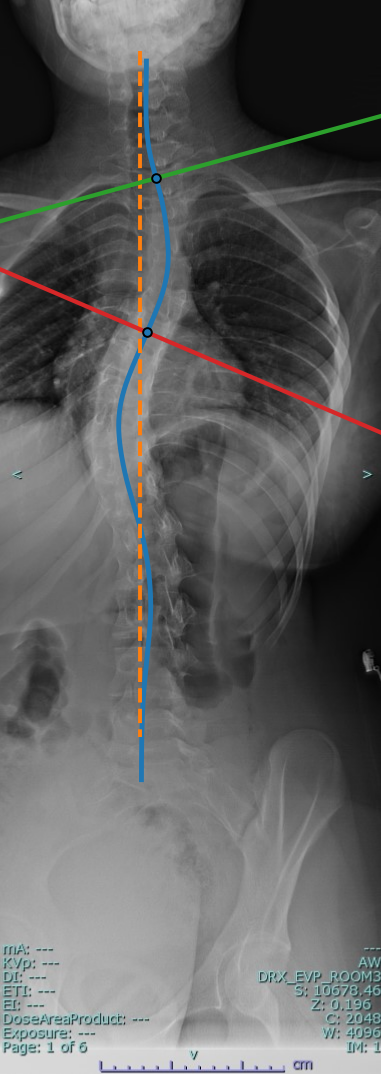
\includegraphics[width=0.27\linewidth]{imagenes/overlay_metrics_21.png}}
\end{tabular}

\caption{Representaciones derivadas del dataset: (c) línea central estimada
de la columna y (d) cálculo del ángulo de Cobb para evaluar la deformidad espinal.}

\label{fig:dataset_metrics}

\end{figure}


\subsection{Preprocesamiento}
\subsection{Arquitectura del modelo}

La arquitectura propuesta integra extracción de características profundas,
representaciones geométricas y modelado contextual global. El objetivo es
capturar tanto patrones locales presentes en las radiografías como la
estructura geométrica global de la columna vertebral.

Sea una radiografía de entrada

\[
I \in \mathbb{R}^{H \times W},
\]

donde \(H\) y \(W\) representan las dimensiones de la imagen.

El pipeline completo del modelo puede representarse como la composición

\[
I
\xrightarrow{\phi}
Z^{cnn}
\xrightarrow{\tau}
Z^{topo}
\xrightarrow{k}
\tilde{Z}
\xrightarrow{\mathcal{T}}
\hat{Y}.
\]

Cada una de estas transformaciones captura diferentes propiedades
estructurales de los datos.

\subsubsection{Extracción de características mediante CNN}

La primera etapa utiliza una red neuronal convolucional para extraer
características espaciales de la radiografía. Formalmente, la CNN define
una función

\[
f_\theta : \mathbb{R}^{H \times W} \rightarrow \mathbb{R}^{n \times d},
\]

que transforma la imagen de entrada en un conjunto de embeddings

\[
Z^{cnn} = f_\theta(I) =
\{z_1, z_2, \dots, z_n\},
\quad z_i \in \mathbb{R}^d.
\]

Estos vectores representan descriptores locales de la anatomía de la
columna vertebral, capturando información de bordes, texturas y patrones
estructurales presentes en la imagen.

\subsubsection{Estructura geométrica y manifold}

Los embeddings generados por la CNN pueden interpretarse como puntos en
un espacio euclidiano de dimensión \(d\)

\[
Z^{cnn} \subset \mathbb{R}^d.
\]

Bajo la hipótesis de variedad, se asume que estos puntos se encuentran
aproximadamente sobre una variedad de menor dimensión

\[
\mathcal{M} \subset \mathbb{R}^d,
\]

la cual describe la geometría intrínseca de la estructura anatómica
presente en la imagen.

Esta interpretación permite estudiar la estructura global de los datos
mediante herramientas geométricas y topológicas.

\subsubsection{Representación topológica mediante complejos simpliciales}

Para capturar relaciones geométricas entre los puntos del embedding se
construye un complejo simplicial utilizando una filtración de
Vietoris--Rips.

Sea

\[
Z = \{z_1,\dots,z_n\}
\]

el conjunto de embeddings. Para un parámetro de escala
\(\varepsilon > 0\), el complejo simplicial se define como

\[
VR_\varepsilon(Z) =
\{\sigma \subseteq Z :
d(z_i,z_j) \le \varepsilon
\ \forall z_i,z_j \in \sigma\}.
\]

Este complejo permite modelar relaciones de conectividad entre los
puntos y capturar propiedades topológicas del conjunto de embeddings.

A partir de esta estructura se obtiene un vector de características
topológicas

\[
Z^{topo} = \tau(VR_\varepsilon(Z)) \in \mathbb{R}^{d_t},
\]

donde \(\tau\) representa un operador de resumen topológico.

\subsubsection{Representación mediante kernels}

Con el objetivo de modelar relaciones no lineales entre los embeddings,
se introduce una función kernel

\[
k(x_i,x_j) =
\langle \Phi(x_i), \Phi(x_j) \rangle_{\mathcal{H}},
\]

donde

\begin{itemize}

\item \(\Phi(\cdot)\) es una función que proyecta los datos en un
espacio de características de mayor dimensión

\item \(\mathcal{H}\) es un espacio de Hilbert con producto interno

\end{itemize}

Esta formulación define un espacio de representación no lineal conocido
como \emph{Reproducing Kernel Hilbert Space} (RKHS).

Algunos kernels utilizados comúnmente son

\[
k_{linear}(x_i,x_j) = x_i^\top x_j
\]

\[
k_{RBF}(x_i,x_j) =
\exp\left(-\frac{\|x_i-x_j\|^2}{2\sigma^2}\right)
\]

\[
k_{poly}(x_i,x_j) =
(x_i^\top x_j + c)^p.
\]

El kernel induce una matriz de similitud

\[
K_{ij} = k(z_i,z_j),
\]

que captura relaciones estructurales entre los embeddings.

\subsubsection{Modelado contextual mediante Transformer}

Los embeddings enriquecidos se procesan mediante un encoder Transformer
que modela relaciones globales entre los diferentes tokens.

Sea

\[
\tilde{Z} = \{\tilde{z}_1,\dots,\tilde{z}_n\}
\]

la secuencia de tokens enriquecidos. El mecanismo de auto-atención se
define como

\[
\mathrm{Attention}(Q,K,V)
=
\mathrm{softmax}
\left(
\frac{QK^\top}{\sqrt{d_k}}
\right)V.
\]

Este mecanismo permite que cada token interactúe con todos los demás
tokens, capturando dependencias globales dentro de la estructura de la
columna vertebral.

\subsubsection{Formulación global del pipeline}

De manera compacta, el modelo completo puede expresarse como

\[
\hat{Y}
=
\mathcal{T}
\left(
k
\left(
\tau
\left(
f_\theta(I)
\right)
\right)
\right).
\]

Esta formulación resume el flujo del modelo: primero se extraen
características locales mediante una CNN, posteriormente se modela la
estructura geométrica de los embeddings mediante complejos simpliciales,
se enriquecen las relaciones entre representaciones mediante kernels y
finalmente un Transformer captura dependencias globales entre tokens.

\begin{figure}[t]
\centering
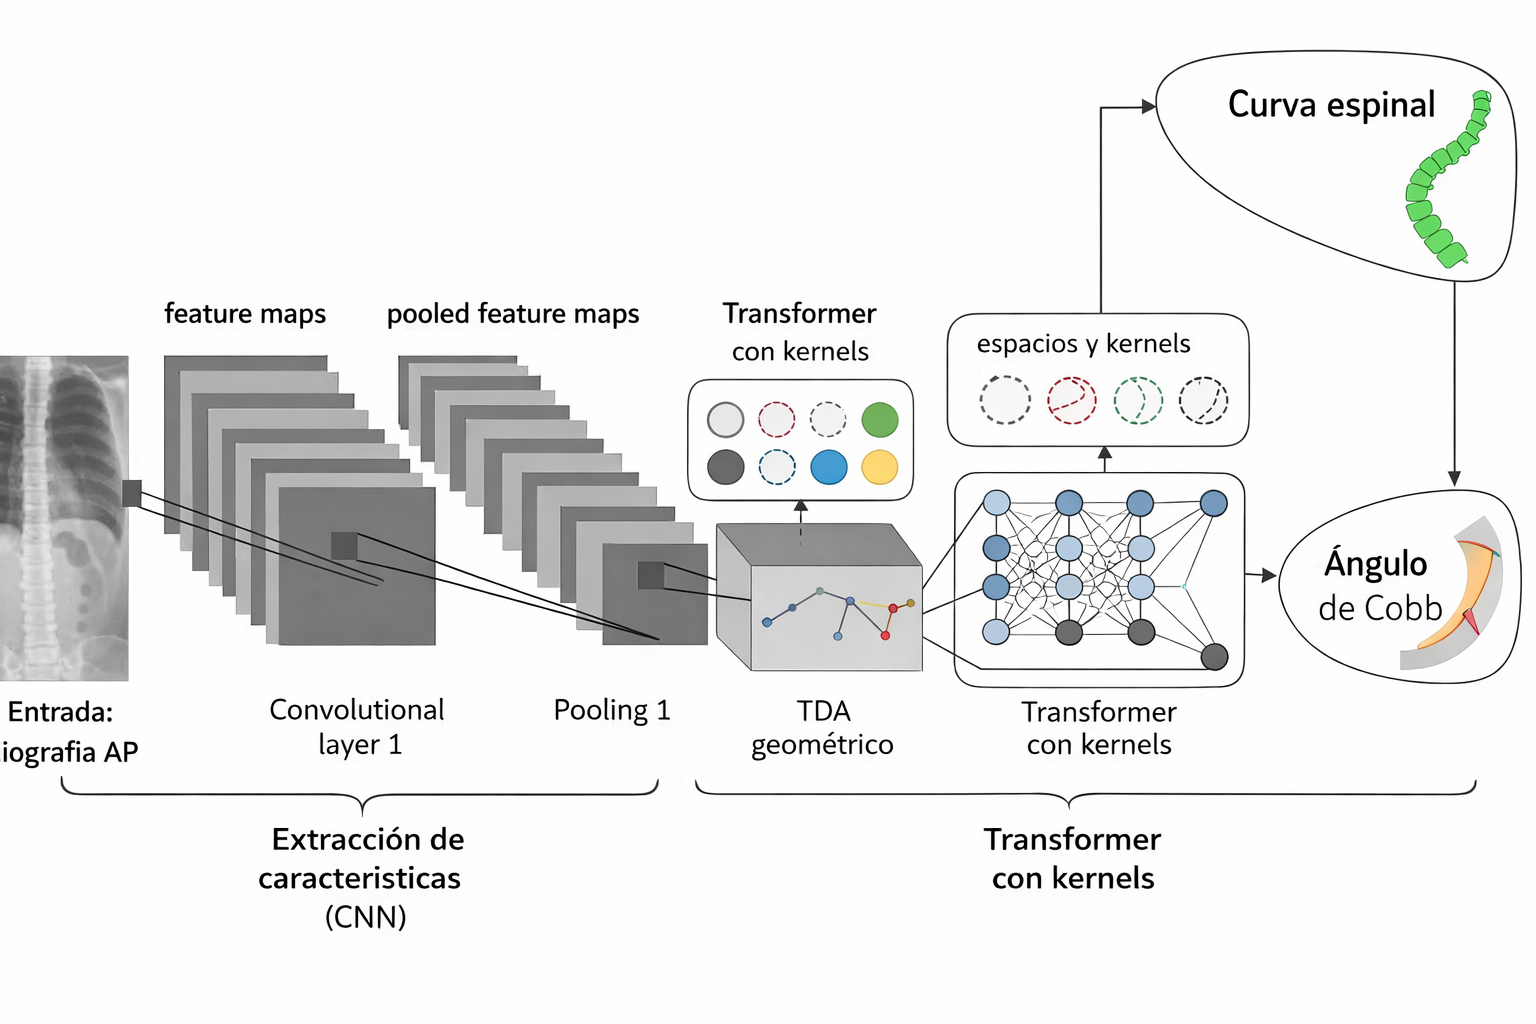
\includegraphics[width=0.9\linewidth]{imagenes/model_architecture.png}
\caption{
Arquitectura general del modelo propuesto. La radiografía de entrada se
procesa mediante una red convolucional que extrae embeddings espaciales.
Estos embeddings se interpretan como puntos en un espacio métrico que
aproximan una variedad geométrica. Sobre este conjunto se construyen
complejos simpliciales para capturar relaciones topológicas entre los
puntos. Posteriormente se aplican funciones kernel para enriquecer el
espacio de representación y finalmente un encoder Transformer modela
las relaciones globales entre tokens para capturar la estructura
completa de la columna vertebral.
}
\label{fig:model_architecture}
\end{figure}

\subsection{Entrenamiento}
\subsection{Métricas de Evaluación}

\section{Resultados}
\section{Análisis}
\section{Discusión}
\section{Conclusiones}
\section{Trabajo Futuro}

\bibliographystyle{IEEEtran}
\bibliography{refs}

\end{document}